\section{Esplorazione: un IPR per i process tensor}\label{sec:ipr}

\CartoonIPR
\subsection{Definizione}
La ``base'' di un process tensor è uno \emph{strumento}: a ogni passo si prepara e si misura il sistema in una certa base. Usiamo la misura proiettiva di S a ogni passo, con lo stato collassato che prosegue nella dinamica. Ne risulta una distribuzione dei record $p(x_1,\dots,x_n)$ su $N=d^n$ storie, con:
\begin{itemize}[leftmargin=1.5em]
\item \textbf{IPR temporale} $\mathcal I_2=\sum_xp(x)^2$, e il suo valore normalizzato $N\mathcal I_2$;
\item \textbf{valori di riferimento}: $N\mathcal I_2=1$ per record uniformi, $\simeq2$ per Porter--Thomas, crescita esponenziale in $n$ per una distribuzione moltiplicativa (log-normale);
\item \textbf{testimone di memoria}. Per un processo Markoviano (prodotto) e uno strumento prodotto con preparazioni fissate, $p$ si fattorizza e $\log\mathcal I_2$ è additivo. La non additività
\[
\Delta I_{\rm rec}=\log_2\frac{\mathcal I_2(\text{tutto})}{\mathcal I_2(\text{passato})\,\mathcal I_2(\text{futuro})}
\]
è quindi un testimone operativo di memoria.
\end{itemize}

\subsection{Risultati esatti nel modello 1}
Senza rumore, la matrice di trasferimento a due repliche per un passo registrato è simmetrica, con autovalori
\[
\lambda_\pm=\frac{D\pm1}{dD\pm1}
\]
sui sottospazi simmetrico e antisimmetrico di E$\otimes$E. Ne segue
\[
\mathcal I_2(n)=\tfrac{1+P_{\rm E}}{2}\,\lambda_+^n+\tfrac{1-P_{\rm E}}{2}\,\lambda_-^n ,
\]
verificato con il Monte Carlo per $D=2,3$, con ambiente puro o misto e con rumore (ricorsione generale), entro $1$--$2\sigma$. Per $D=1$ si ritrova il prodotto di fattori Porter--Thomas, $N\mathcal I_2=(2d/(d+1))^n$.

\begin{figure}[t]
\centering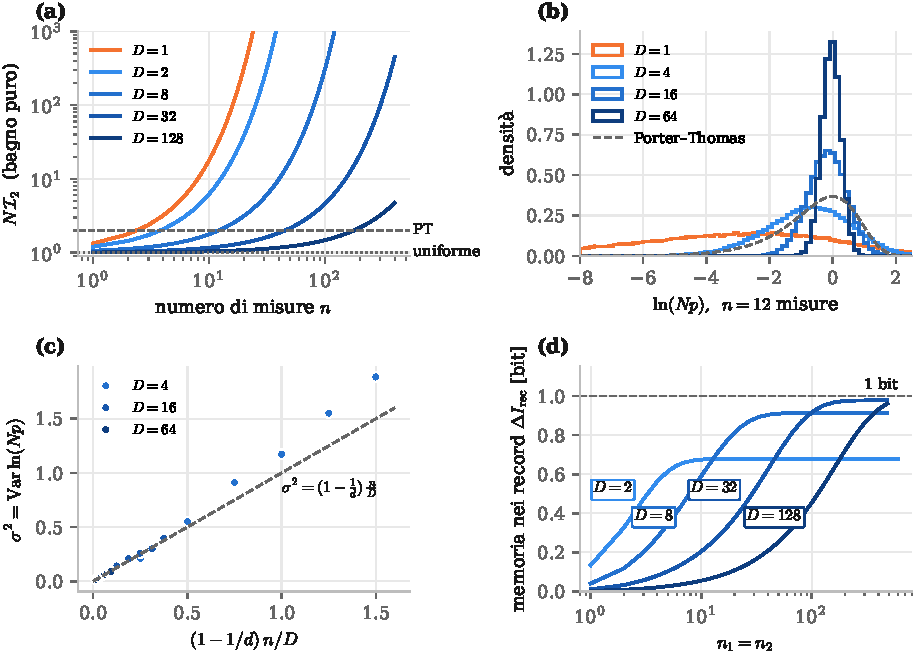
\includegraphics[width=\textwidth]{figs/fig_ipr.pdf}
\caption{IPR temporale nel modello 1 ($d=2$). (a) IPR normalizzato $N\mathcal I_2$ con bagno puro: 1 corrisponde a record uniformi, 2 a Porter--Thomas. Senza bagno ($D=1$) la crescita esponenziale è immediata; con un bagno grande i record restano quasi uniformi fino a $n\sim D$. (b) Istogrammi di $\ln(Np)$ a $n=12$ (Monte Carlo): sono log-normali e si stringono al crescere di $D$; tratteggiata la Porter--Thomas. (c) Collasso della varianza su $\sigma^2=(1-1/d)\,n/D$. (d) Memoria vista nei record, $\Delta I_{\rm rec}$: satura sotto 1 bit, mentre la memoria quantistica è $2\log_2D$, cioè 2, 6, 10 e 14 bit per $D=2,8,32,128$.}
\label{fig:ipr}
\end{figure}
\paragraph{La distribuzione temporale è log-normale (\cref{fig:cartoon-ipr,fig:ipr}).} Con il Monte Carlo sulle probabilità dei record (bagno puro, $d=2$):
\begin{itemize}[leftmargin=1.5em]
\item $\ln(Np)$ ha varianza $\sigma^2\simeq(1-\tfrac1d)\,n/D$ (pendenza misurata $0.58$, $0.52$, $0.51$ volte $1/D$ per $D=4,16,64$) e media $-\sigma^2/2$;
\item vale $N\mathcal I_2=e^{\sigma^2}=(d\lambda_+)^n$, e la media quenched coincide con quella annealed per $D\ge4$;
\item per $D=1$ la varianza cresce di circa $1.1$ per passo.
\end{itemize}
La distribuzione dei record è quindi \emph{moltiplicativa}, cioè ``Markoviana'' nel senso di prodotto di fattori. Non è mai Porter--Thomas. Il bagno rende i fattori quasi uniformi: i record restano quasi uniformi fino a
\[
n^*\simeq\ln2\,\frac{dD+1}{d-1}\qquad(N\mathcal I_2=2),
\]
dopodiché si allargano. La dimensione efficace del bagno si legge dal record di una sola sonda, tramite $\sigma^2/n=(1-1/d)/D$.

\paragraph{I record vedono poca memoria.} $\Delta I_{\rm rec}$ (annealed) satura a meno di 1 bit: $0.68$, $0.91$, $0.98$ bit per $D=2,8,32$, raggiunti su tempi $\sim D$. La memoria quantistica Rényi-2 è invece $2\log_2D$ (\cref{sec:model1}). Quasi tutta la memoria del process tensor è invisibile ai record in una base fissata. Il valore limite di 1 bit va verificato con medie quenched.

\paragraph{Bagno a temperatura infinita.} Con $P_{\rm E}=1/D$ le deviazioni dai record uniformi sono $O(n^2/D^2)$ invece che $O(n/D)$: a $n=4$, $N\mathcal I_2=1.039$ per $D=8$ misto contro $1.257$ per $D=8$ puro.

Questo è un caso di un fatto generale. Per un bagno scramblante grande a temperatura infinita, tutte le statistiche dei record ($\sum_xp^k$) coincidono con quelle del processo medio (una replica) a meno di correzioni $O(1/D^2)$. Il motivo è che i record legano le repliche solo sulle gambe di S, mentre E è tracciato replica per replica a entrambi i capi.

Lo stesso argomento dice che nel modello 2 a $D=\infty$ i record sono una catena di Markov classica, generata dal canale a una replica: tutta la fisica dell'eco è invisibile ai record.

\paragraph{Rumore.} Con rumore locale sull'ambiente sia la crescita di $N\mathcal I_2$ sia $\Delta I_{\rm rec}$ calano esponenzialmente in $L$. Per i record non abbiamo visto una transizione netta.

\subsection{La questione della base}
\begin{enumerate}[leftmargin=2em]
\item \textbf{Modelli Haar} (modello 1). La base è irrilevante per invarianza.
\item \textbf{Modelli strutturati} (collo di bottiglia, dual-unitari, Floquet). A $D$ grande la base entra solo tramite il canale a una replica. Le basi allineate ai modi lenti di $\mathcal M$ massimizzano le correlazioni temporali dei record.
\item \textbf{Versione indipendente dalla base.} Con preparazioni e misure in basi Haar indipendenti su ogni gamba, la media dell'IPR è
\[
\mathbb E_U\,\mathcal I_2=(d+1)^{-2n}\sum_{A\subseteq\text{gambe}}\operatorname{Tr}\Upsilon_A^2 .
\]
È l'analogo multi-tempo della formula delle misure randomizzate, e lega l'IPR temporale alle purezze dei marginali di $\Upsilon$, quindi a $I_2$.
\item \textbf{Base di operatori.} L'IPR della distribuzione di Pauli di $\Upsilon$, $\Xi(P)\propto\operatorname{Tr}(\Upsilon P)^2$, è un'entropia stabilizer del processo, cioè ``magia temporale''. È invariante per Clifford e naturale per WP-A; non l'abbiamo ancora calcolato.
\end{enumerate}

\subsection{Cosa ci sembra promettente}
\begin{itemize}[leftmargin=1.5em]
\item \textbf{Statistica log-normale dei record come sonda di bagni finiti.} Estrarre $D_{\rm eff}$ dalla crescita di $\sigma^2$ in modelli strutturati e in catene caotiche, a $D$ finito, dove i record vedono memoria.
\item \textbf{Test di Markovianità sui record.} Confrontare $p$ con la migliore catena di Markov, usando la mutua informazione condizionata di Shannon fra passato e futuro dato il presente. Va a zero a $D=\infty$ (modello 2); misurarne le correzioni $O(1/D)$.
\item \textbf{IPR di Pauli del process tensor.} È a quattro repliche ed è legato al doping.
\item \textbf{Record con eco.} Protocolli in cui i record legano le repliche anche dentro E, come le misure dell'ambiente o gli echi. Lì l'IPR temporale vede la fisica del settore $\circ$.
\end{itemize}
